


\chapter{Preliminaries}\label{sec:preliminaries}

\section{Motivation}\label{sec:motivation}

Brain–Computer Interfaces (BCIs) have emerged as a powerful class of technologies that enable direct communication between the brain and external devices. These systems are increasingly being applied in neurorehabilitation, education, and clinical diagnosis due to their ability to monitor and interpret neural activity in real time. BCIs have the potential to revolutionize the way cognitive states are assessed and modulated by offering closed-loop interaction mechanisms that adapt to the user’s brain dynamics \cite{Lim2023,Lin2025}. Central to this capability is the choice of neuroimaging modality, which must meet strict criteria in temporal resolution, portability, and cost-effectiveness—especially in applications involving children or naturalistic settings.

Several neuroimaging techniques have been explored for use in Brain–Computer Interface (BCI) systems, each with distinct advantages and limitations. Functional Magnetic Resonance Imaging (fMRI) offers high spatial resolution and whole-brain coverage, but its cost, immobility, and dependence on specialized facilities make it impractical for real-time interaction or integration with everyday environments \cite{Yang2025}. Magnetoencephalography (MEG) provides excellent spatiotemporal resolution but is similarly constrained by high operational costs and the need for magnetically shielded rooms \cite{Peksa2023}. Functional Near-Infrared Spectroscopy (fNIRS), a more portable option, measures cortical hemodynamic responses with moderate spatial resolution and tolerance to movement \cite{Doherty2023}. However, its low temporal resolution limits its ability to capture fast-changing neural dynamics, such as those required for attentional monitoring or neurofeedback.

Electroencephalography (EEG), by contrast, emerges as the most suitable modality for BCI applications that demand real-time responsiveness, portability, and affordability. EEG records the brain's electrical activity through non-invasive scalp electrodes, offering millisecond-level temporal resolution ideal for tracking rapid cognitive events like attention shifts or inhibitory control. While EEG's spatial resolution is lower compared to fMRI or MEG, advances in signal processing—such as QEEG, functional connectivity analysis, and source localization—have greatly enhanced its ability to extract meaningful neurophysiological markers \cite{Caiado2025,Yadav2023, Varbu2022}. Moreover, EEG's lightweight hardware, low infrastructure requirements, and compatibility with embedded systems make it an ideal foundation for interactive, portable, and scalable BCI solutions.

\begin{figure}[h]
 \centering
 \includegraphics[width=1\textwidth]{Figures/Neuroimagrre.pdf}
 \caption{Comparison of neuroimaging modalities by spatial resolution, temporal resolution, and cost. EEG stands out for its affordability, portability, and millisecond-level responsiveness.}
 \label{fig:neuroimaging_comparison}
\end{figure}

One of the most compelling clinical applications of EEG-based BCIs is in the assessment and intervention of neurodevelopmental disorders such as Attention Deficit Hyperactivity Disorder (ADHD). ADHD affects approximately 10\% of children in Colombia \cite{salari2023global,pineda2003prevalence} and is characterized by persistent symptoms of inattention, hyperactivity, and impulsivity that interfere with academic performance, social relationships, and emotional regulation. Conventional diagnostic practices rely heavily on behavioral questionnaires and clinical observation, which, while informative, are inherently subjective and susceptible to bias \cite{raiker2017accuracy}. In this context, EEG offers a valuable alternative by enabling the objective measurement of neural correlates linked to attention and impulse control. Well-established EEG biomarkers such as elevated theta/beta ratios and altered event-related potentials (e.g., P300) have been extensively validated in the ADHD literature, making EEG a scientifically robust and clinically relevant tool for real-time cognitive monitoring and neurofeedback interventions.

Serious games are digital environments designed not solely for entertainment, but to fulfill educational, therapeutic, or cognitive objectives. In the context of neurodevelopmental disorders such as ADHD, they have become increasingly relevant as tools for both cognitive assessment and intervention \cite{Patino2025}. Their engaging and adaptive nature allows them to target specific executive functions—like attention, inhibition, and working memory—while maintaining high user motivation, particularly among children \cite{RodriguezTimana2024}. These features make serious games particularly compatible with EEG-based BCIs for interactive cognitive modulation.


Serious games designed for ADHD not only provide engaging environments for cognitive stimulation, but also serve as structured frameworks for assessing and training specific executive functions. Two principal paradigms guide the design of these games. The first is the task-based paradigm, which integrates classical neuropsychological tasks—such as the Go/No-Go, n-back, or Stroop test—into interactive game mechanics. This allows for the precise measurement of behavioral responses tied to well-established cognitive models \cite{Fang2025}. The second is the neurofeedback paradigm, in which the game dynamically responds to real-time EEG signals, offering auditory or visual feedback based on the user’s brain state. This paradigm supports operant conditioning mechanisms, encouraging users to self-regulate neural activity linked to attentional control and inhibition \cite{Firouzabadi2022}. 

These paradigms are often aligned with four core cognitive models critical to ADHD pathology: attention, working memory, inhibition, and planning. Games targeting the attentional model aim to improve sustained and selective attention, often requiring players to maintain focus amid distractions or shifting stimuli \cite{Chen2024}. Working memory is typically trained through tasks that require the temporary storage and manipulation of information, such as remembering sequences or updating mental representations. The inhibition model involves suppressing prepotent responses or resisting distractions—commonly implemented through fast-paced decision-making challenges or impulse control mechanics \cite{Takahashi2024, BreitlingZiegler2020}. Finally, the planning model emphasizes goal-directed behavior, encouraging users to sequence actions, solve multi-step problems, or anticipate future outcomes \cite{Lorini2022}. By aligning game mechanics with these cognitive models, serious games become powerful tools not only for engagement but for targeted neurocognitive intervention, particularly when combined with EEG-based BCIs that provide objective feedback on brain performance in real time.


\begin{figure}[h]
 \centering
 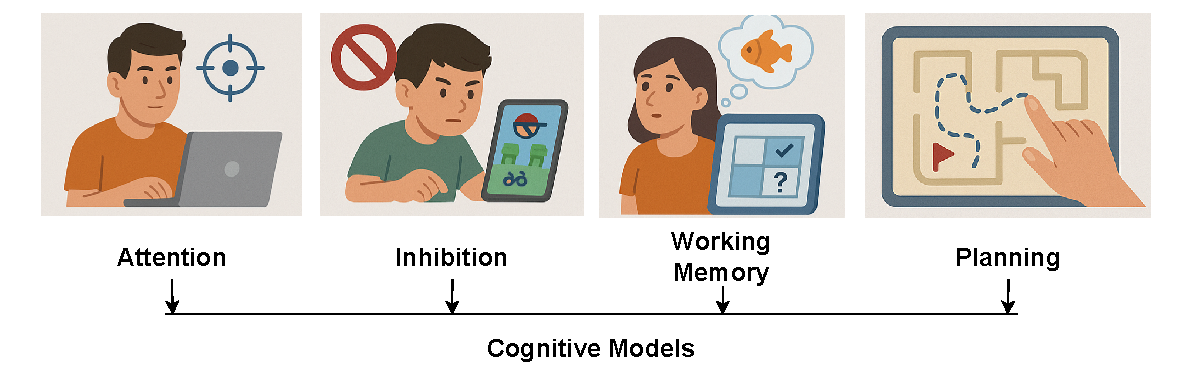
\includegraphics[width=1\textwidth]{Figures/cognitive.pdf}
 \caption{Core cognitive models targeted by serious games in ADHD interventions: attention, working memory, inhibition, and planning. Each model maps to a specific set of game dynamics and EEG markers.}
 \label{fig:cognitive_models}
\end{figure}



Serious games integrated with BCI technology have demonstrated therapeutic benefits by reinforcing executive function, improving behavioral outcomes, and reducing symptom severity through active attention training and neurofeedback mechanisms \cite{Doulou2025}. Active BCIs, in which users intentionally modulate their focus to influence the outcome of the game, have been shown to strengthen cognitive control and promote long-term neuroplastic changes relevant to ADHD pathology \cite{Cervantes2023}. These platforms also enable adaptive feedback, allowing interventions to dynamically adjust to each child's neurocognitive profile.

However, the effectiveness of such systems depends on precise temporal synchronization between game-generated stimuli and EEG signals. Detecting event-related potentials (such as the P300 wave) or dynamic oscillations in the theta and beta frequency bands during attentional tasks requires sub-millisecond timing accuracy \cite{Wikstrom2022, Sandstrak2024}. Without rigorous synchronization—typically achieved via TTL triggers or low-latency USB/Wi-Fi communication—EEG signal interpretation is susceptible to noise, jitter, and event misclassification \cite{iwama2023two}. This challenge is particularly critical in real-time therapeutic environments where accurate feedback is essential.

Recent developments in portable EEG hardware have expanded the applicability of BCIs for ADHD beyond clinical settings, enabling real-time monitoring and feedback in homes, classrooms, and therapeutic environments. Low-cost, wireless EEG headsets—equipped with dry electrodes and embedded microcontrollers—have been successfully integrated into neurofeedback systems and serious games designed for children \cite{Xu2018}. These platforms allow for real-time signal acquisition and onboard processing, supporting closed-loop interventions without reliance on external computers. Thanks to ARM-based processors and system-on-chip (SoC) designs, it is now possible to run lightweight machine learning models directly on the device for real-time EEG classification \cite{Wang_2020}. Moreover, custom head-mounted EEG systems have shown reliable tracking of the theta/beta ratio, a key biomarker for ADHD, during interactive tasks \cite{Larocco2020}.

Altogether, these technological advances offer a promising foundation for rethinking ADHD diagnosis and intervention—especially in child populations. Nevertheless, critical technical challenges remain, particularly the synchronization of cognitive stimuli with neurophysiological responses in embedded systems. This challenge motivates the present research, which aims to design and implement a portable EEG acquisition and analysis system with precise synchronization to game events, enabling objective, real-time support for cognitive stimulation and diagnostic processes in children with ADHD.




